\chapter{Invasive Computing}
\label{chapter:invasive computing}
Invasive Computing is a novel paradigm for designing and programming future parallel systems. Decreasing feature sizes are motivating a redesign of multi million transistor system-on-chip architectures. This can lead to a dramatic increase in the rates of temporary and permanent faults as well as feature variations. SoCs with 1000 or more processors on a single chip in the year 2020 are foreseen, hence static and central management concepts to control the execution of all resources are no longer appropriate. Invasive Computing allows a program to be resource-aware by which it can explore and dynamically spread its computations to neighbour processors in a phase called as \textbf{\textit{invade}}, then to execute portions of code of high parallelism degree in parallel based on the available invasible region in a given multi-processor architecture in a phase called as \textbf{\textit{infect}}. Later, once the degree of parallelism should be lower again or if it terminates, the program may enter a \textbf{\textit{retreat}} phase where it can deallocate resources and resume execution again, for example, on a single processor. With the help of such resource awareness, the program has the ability to self-organise itself and be immune to faults, feature variations, be highly scalable, show performance gain and record a higher resource utilization metric.\\ \\
This concept would require not just new programming concepts, languages, compilers and operating systems but a radical change in the architectural design of MPSoCs(\textit{Multi-Processor Systems-On-a-Chip}) so as to efficiently support invasion, infection and retreat operations. Some of the main motivations behind the idea of invasive computing are enumerated below:
\begin{itemize}
\item \textbf{\textit{Programmability}} How to map algorithms and programs to 1000 processors or more and how to benefit from the massive parallelism available by tolerating manufacturing defects, feature variations etc.
\item \textbf{\textit{Adaptivity}} Modern applications have unpredictable resource requirements most of which may not be known at compile-time. In addition to this, when different applications are running on a single chip, resource distribution will have to happen dynamically keeping up a high resource utilization and performance. These factors show the need for some sort of hardware / software reconfigurability of the MPSoC.
\item \textbf{\textit{Scalability}} How to efficiently run algorithms and programs on different number of resources?
\item \textbf{\textit{Physical Constraints}} Heat dissipation will be a major bottleneck. Intelligent methods and architectural support to run algorithms at different speeds to exploit parallelism under power reduction is needed.
\item \textbf{\textit{Reliability and Fault-Tolerance}} Applications must be immune to temporal or permanent faults that may be caused due to manufacturing defects, feature variations, degradation etc. This especially has a higher likelihood to happen in the case of future MPSoCs.
%%%%%%%
\end{itemize}
The paradigm of invasive computing offers a new perspective for programming large scale HPC systems. Current resource management systems manage resources via static partitioning among parallel jobs. This is a very rigid approach considering that an application will then be limited to a fixed amount of parallelism it can utilize. This, however, will not be beneficial especially in the case of future exascale systems where if one needs to derive maximum performance then the maximum number of resources will have to be allocated. The application can benefit from invasive programming during certain phases of its runtime by running at maximum parallelism and in the remaining time it can run at a lower parallelism.\\ \\
%%%%%%%
Another motivation is for a specific classes of applications like multi-grid and adaptive grid. Multi-grid applications work on multiple grid levels ranging from fine to coarse grids. On fine grids, more resources could yield better performance and efficiency, whereas on coarse grids fewer resources would be sufficient. In the case of adaptive grid applications, the grid is dynamically refined according to the current solution and the application may go through different levels of parallelism in different phases.\\ \\
%%%%%%%
Scaling the systems to exaflop level would consume significantly more power that would very likely cross a gigawatt. Reducing the power requirement by a factor of atleast 100 is a challenge for future hardware and software technologies. Invasive computing concept with invasive programming models combined with intelligent resource management and flexible scheduling mechanisms can possibly help in addressing this challenge.\\ \\
%%%%%%%
Coping with run-time errors would be another major challenge. Due to design and power constraints, the clock frequency is unlikely to change and feature sizes would continue to decrease as per moore's law for the next few years. By 2020, it is envisaged that exascale systems can possibly have approximately one billion processing elements. An immediate consequence is that the frequency of errors will increase while timely identification and correction of errors would be much more difficult. Fault tolerance would be one of the most important challenges in this regard.\\ \\
%%%%%%%
Exploiting massive parallelism for current and emerging scientific applications would also be another major challenge.
\section{Traditional Resource Management}
The role of a resource manager is to act like a \textit{glue} for a parallel computer to execute parallel jobs. MPI would typically be used to manage communications within the parallel program. A resource manager allocates resources within a cluster, launches and otherwise manages the jobs. The combination of \textit{Scheduler}$+$\textit{Resource Manager} makes it possible to run parallel jobs and is together termed as a Batch System. These systems are classified depending on whether they work towards serving job requests to satisfy the available resources or they also plan for the future<ref>.
%%%%%%
\subsection{Classification}
The process of computing a schedule may be done by a queueing or planning based scheduler. A \textit{Schedule} is computed for the job requests that are present in the job queue. Every request contains information such as the number of requested resources and a duration for how long the resources are requested for. There can also be some reservation requests present. These request for resources at a specified time for a given duration. Once the scheduler accepts such a request, it is a reservation and those exact resources are then blocked for that specified time and are unavailable for any scheduling purposes.\\ \\
%%%%%%
Queuing systems try to utilize the currently available resources in order to satisfy the job requests. Future resource planning for all the pending requests is not done. Hence, the pending requests have no proposed start times. Planning systems in contrast, plan for the present and the future. Planned start times are assigned to all requests and a complete schedule about the future resource usage is computed.\\ \\
%%%%%%%%%%%%
\textbf{\textit{Queuing Systems }} These systems have several queues with different limits on the number of requested resources and the runtime limit for the job. Jobs within a queue are ordered according to a scheduling policy, e. g. FCFS (first come, first serve). Queues might be activated only for specific times (e. g. prime time, non prime time, or weekend). The task of a queuing system is to assign free resources to waiting requests. The highest prioritized request is always the queue head. If it is possible to start more than one queue head, further criteria like queue priority or best fit (e. g. leaving less resources idle) are used to select a request. There might also exist a high priority queue whose jobs are preferred at any time. If not enough resources are available to start any of the queue heads, the system waits until enough resources become available. These idle resources may be utilized with less prioritized requests by backfilling mechanisms.\\ \\
%%%%%%%
In queuing systems, no information about future job starts are available. Consequently guarantees can not be given and resources can not be reserved in advance. Resource reservation will have to be done manually by the administrative staff. Job requests also come with run time limits. If a job runs for more than the run time limit it specified or the partition limit, then the system will usually kill such a job.\\ \\
%%%%%%%%%
\textbf{\textit{Planning Systems }}Planning systems schedule for the present and future. They assign start times to all requests and a full schedule is generated. Runtime estimates for jobs are mandatory for this planning. With this knowledge advanced reservations are easily made possible. The re-planning process is the key element of a planning system. Each time a new request is submitted or a running request ends before it was estimated to end, a new schedule has to be computed and this function is invoked. At the beginning of a re-plan, All pending requests are sorted according to a scheduling policy in addition to clearing their previously planned start times. All the pending requests are then re-inserted at the earliest possible start time in the schedule. After this step each request is assigned a planned start and end time.\\ \\
%%%%%%%%%
As planning systems work with a full schedule and assign start times to all requests, resource usage is guaranteed and advanced reservations are possible. If any reservation request is accepted then it is stored in an extra list for accepted reservations. During the re-planning process this list is processed before the list of standard job requests which can float around in the schedule. One drawback in a planning system is the cost of scheduling.
%%%%%%%%%
\subsection{Job Scheduling}
Typical resource management systems store job requests in list-like structures. A scheduling policy consists of two parts: inserting a new request in the data structure at its submission and taking requests out during the scheduling. Different sorting criteria are used for inserting new requests and some examples are (either in increasing or decreasing order):
\begin{itemize}
\item by arrival time: FCFS (first come first serve). 
\item by duration: Both increasing and decreasing orders are used. Sorting by increasing order leads to SJF (shortest job first). Accordingly LJF (longest job first) sort by decreasing run time. This requires job runtime estimates. SJF and LJF are both not fair, as very long (SJF) and short (LJF) jobs potentially wait forever.
\item by area: The jobs area is the product of the width (requested resources) and length (estimated duration). 
\item by given job weights: Jobs may come with weights which are used for sorting. Job weights consist of user or system given weights or a combination of both. For example: all jobs receive default weights of one and only very important jobs receive higher weights, i. e. they are scheduled prior to other jobs.
%\item by the Smith ratio: The Smith ratio of a job is defined by weight area and is used in the PSRS (Preemptive Smith Ratio Scheduling) algorithm [75].
\item by many others: e. g. smith ratio, number of requested resources, current slowdown, ...
\end{itemize}

In the scheduling process, Jobs are taken out of the ordered data structure for either a direct start in queuing systems or for placing the job in a full schedule (planning system):
\begin{itemize}
\item front: The first job in the data structure is always processed. Most scheduling policies use this approach as only with this a sorting policy makes sense. FCFS, SJF, and LJF use this approach.
\item first fit: The first job that fits into the available resources.
\item best fit: All jobs are tested to see whether they can be scheduled. According to a quality criterion the best suited job is chosen. Commonly the job which leaves the least resources idle in order to increase the utilization is chosen. If more than one job is best suited an additional rule is required, e. g. always take the first, the longest/shortest job, or the job with the most weight.
\end{itemize}
%%%%%%%
If fairness in common sense has to be met, i. e. the starting order equals the arrival order, only the combination of sorting by increasing arrival time and always processing the front of the job structure can be used. All other combinations do not generate fair schedules. However, such a fair scheduler is not very efficient, as jobs usually have to wait until enough free resources are available. Therefore, basic scheduling policies are extended by backfilling, a method to avoid excessive idleness of resources.\\ \\
%%%%%
\textbf{\textit{Backfilling }}The default algorithms used by job schedulers for parallel supercomputers select jobs for execution in FCFS order, and run each job to completion, in batch mode. The problem with this simplistic approach is that it causes significant fragmentation, as jobs with arbitrary sizes/arrivals do not pack perfectly. Specifically, if the first queued job requires many processors, it may have to wait a long time until enough are freed. During this time, processors stand idle as they accumulate, despite the fact there may very well be enough of them to accommodate the requirements of other, smaller, waiting jobs.\\ \\
%%%%%
To solve the problem, most schedulers therefore employ the following algorithm. Whenever the system status changes (job arrivals or terminations), the scheduler scans the queue of waiting jobs in order of arrival (FCFS) and starts the traversed jobs if enough processors are available. Upon reaching the first queued job that cannot be started immediately, the scheduler makes a reservation on its behalf for the earliest future-time at which enough free processors would accumulate to allow it to run. This time is also called the \textit{shadow time}. The scheduler then continues to scan the queue for smaller jobs (require fewer processors) that have been waiting less, but can be started immediately without interfering with the reservation. In other words, a job is started out of FCFS order only if it terminates before the shadow time and therefore does not delay the first queued job, or if it uses extra processes that would not be needed by the first queued job. The action of selecting smaller jobs for execution before their time provided they do not violate the reservation constraint is called backfilling.\\ \\
\begin{figure}[!htbp]
\centering
\includegraphics[width=1.0\textwidth, height=45mm]{./figures/"FCFS+Backfilling".pdf}
\caption{FCFS with and without Backfilling}
\label{fig:32}
\end{figure}
This approach was initially developed for the IBM SP1 supercomputer installed at the Argonne National Laboratory as part of EASY (Extensible Argonne Scheduling System), which was the first backfilling scheduler [ref]. In terms of performance, backfilling has shown to be a close second to more sophisticated algorithms that involve preemption (time slicing), migration, and dynamic partitioning [ref]. The down side of backfilling is that it requires the scheduler to know in advance how long each job(\textbf{\textit{user runtime estimates}}) will run. This is needed for two reasons:
\begin{itemize}
\item to compute the shadow time for the longest-waiting job (e.g. in the example given in \ref{fig:32}, we need to know the runtimes of job 1 and job 2 to determine when their processors will be freed in favor of job 3), and
\item to know if smaller jobs positioned beyond the head of the wait-queue are short enough to be backfilled (we need to make sure backfilling job 4 will not delay job 3, namely, that job 4 will terminate before the shadow time of job 3).
\end{itemize}
Jobs that exceed their estimates are killed, so as not to violate subsequent commitments (the reservation). The combination of simplicity, effectiveness, and FCFS semantics has made EASY a very attractive and a very popular job scheduling strategy. Nowadays, virtually all major commercial and open-source production schedulers support EASY backfilling. Figure \ref{fig:3} briefly mentions some of the various tunable knobs of backfilling algorithms.
\begin{figure}[!htbp]
\centering
\includegraphics[width=1.0\textwidth, height=190mm]{./figures/"BackfillParameters".pdf}
\caption{Backfilling Variations}
\label{fig:3}
\end{figure}
%%%%%%%
\subsection{SLURM}
The prime focus of this work will be on \textbf{SLURM(Simple Linux Utility For Resource Management)} which will be the choice of batch system upon which the support for Invasive Computing will be demonstrated. SLURM is a sophisticated open source batch system written in C whose development started in the year 2002 at Lawrence Livermore National Laboratory as a simple resource manager for Linux Clusters. A few years ago it spawned into an independent firm under the name SchedMD. SLURM has since its inception also evolved into a very capable job scheduler through the use of optional plugins. It is used on many of the world's largest supercomputers and is used by a large fraction of the world's TOP500 Supercomputer list. It supports many UNIX flavors like AIX, Linux, Solaris and is also fault tolerant, highly scalable, and portable.\\ \\
\begin{figure}[!ht]
\centering
\includegraphics[width=1.0\textwidth, height=150mm]{./figures/"SLURM Architecture".pdf}
\caption{SLURM Architecture}
\label{fig:6}
\end{figure}
%%%%%
\noindent
SLURM has a centralized manager called \textbf{\textit{slurmctld}}(controller daemon) that is the main nerve center of SLURM. SLURM operates in a style simlar to the Master-Slave paradigm where the Master is the \textbf{\textit{slurmctld}}. It takes centralized decisions to monitor resources and work. In the event of a failure, there may also be a backup controller. Each of the nodes in the cluster has a daemon running on it called as \textbf{\textit{slurmd}} and these are the slaves. These daemons are started on every node and they are responsible for monitoring them. This can resemble a remote shell: it waits for work from the controller, executes that work, returns status and waits for more work. The \textit{slurmd} daemons provide fault-tolerant hierarchical communications and also are responsible for spawning an additional daemon called \textbf{\textit{slurmstepd}}. The step daemon as it is called is responsible for the node local part of the job step that are the subset of processes running on the local node. A job step in SLURM refers to an application started with the help of srun and its allocated resources. srun could be used independently to launch jobs or one can specify the same within a batch script while using sbatch. \textbf{\textit{srun}} is one of the tools SLURM provides that allows the user to launch interactive jobs on the cluster, \textbf{\textit{sbatch}} to launch batch jobs and several others relating to accounting, job status, cancellation operation etc.\\ \\
The figure \ref{fig:6} shows the high level architecture of SLURM with the interaction between the several of its key components. It also shows the interaction between an MPI application through the PMI(Process Management Interface), \textit{slurmd} daemon of a node and the \textit{slurmstepd}.
\textbf{Plugins} are dynamically linked objects loaded at run time based upon configuration file and/or user options. Approximately $80$ plugins of different varities are currently available. Some of them are listed below:
\begin{itemize}
\item \textbf{\textit{Accounting storage:}} MySQL, PostgreSQL, textfile.
\item \textbf{\textit{Network Topology:}} 3D-Torus, tree.
\item \textbf{\textit{MPI:}} OpenMPI, MPICH1, MVAPICH, MPICH2, etc.
\end{itemize}
PLugins are typically loaded when the daemon or command starts and persist indefinitely. They provide a level of indirection to a configurable underlying function.
%\begin{figure}[!htbp]
%\centering
%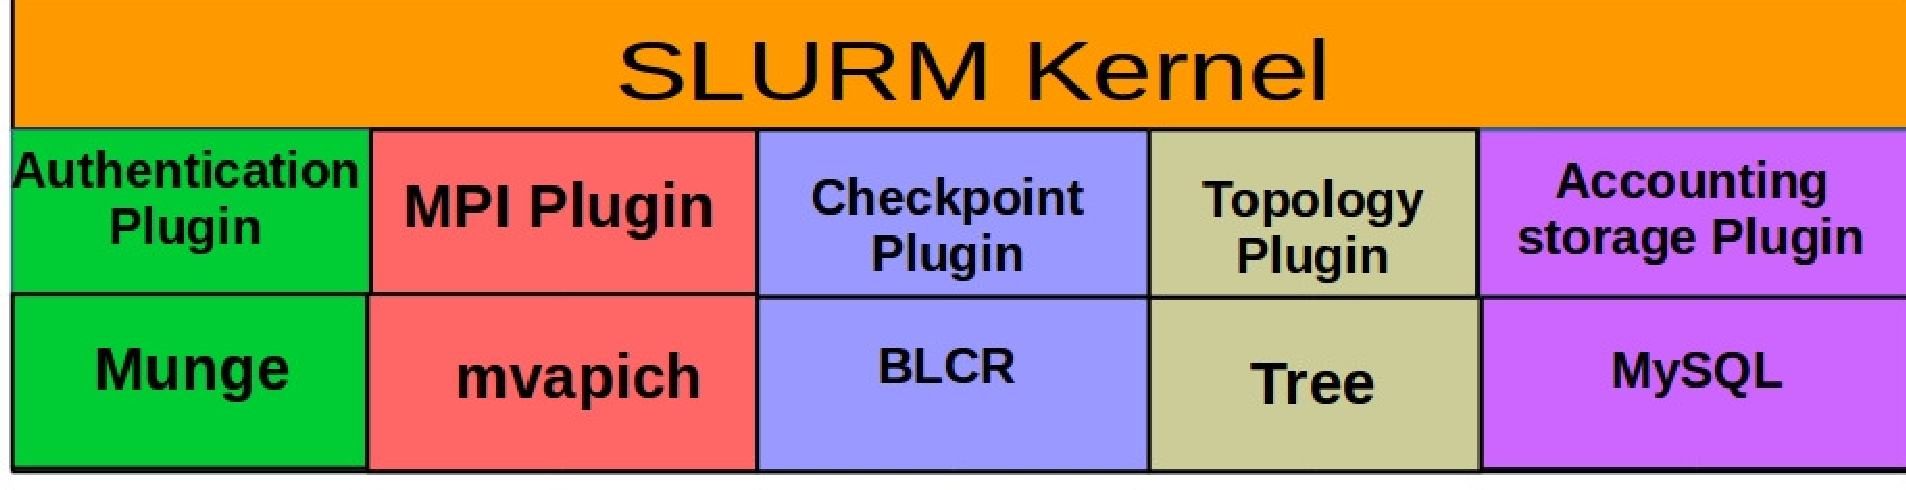
\includegraphics[width=1.0\textwidth]{./figures/plugin.pdf}
%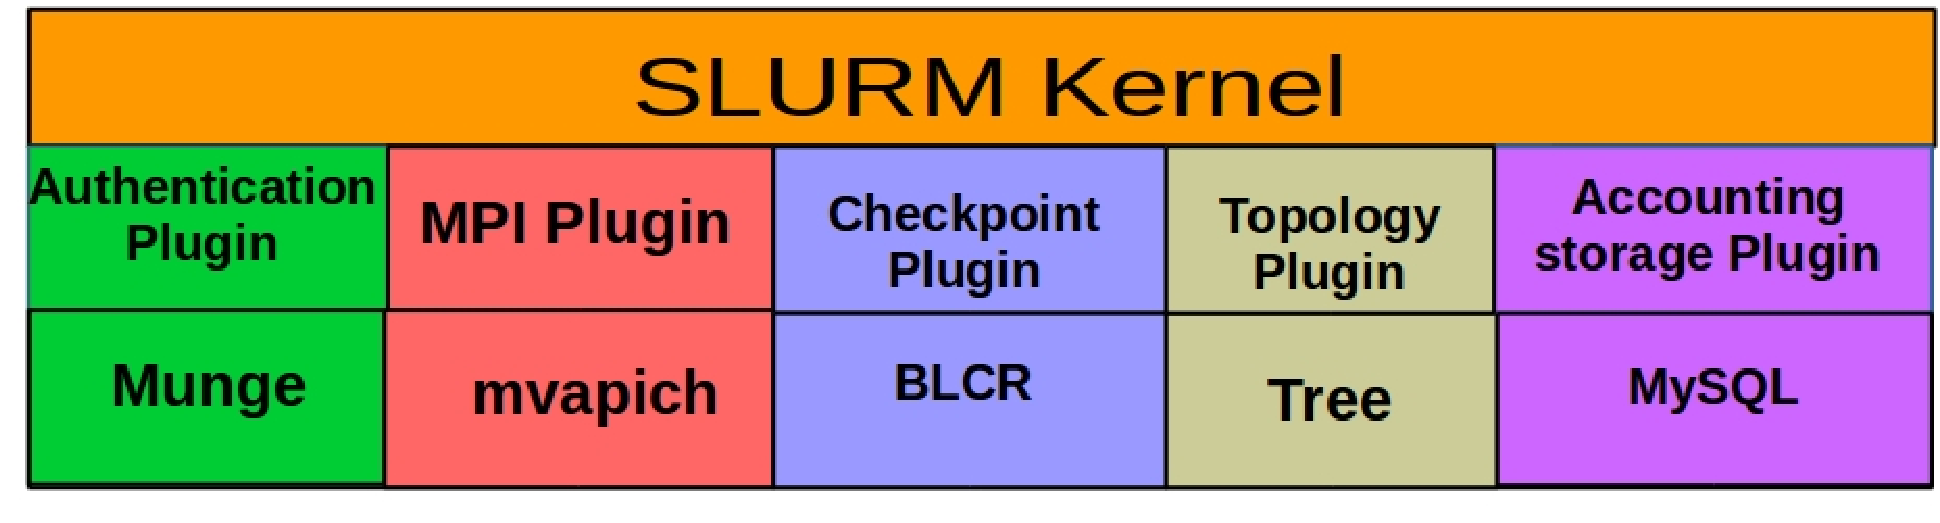
\includegraphics[width=1.0\textwidth]{./figures/plugin.eps}
%\vspace{-0.15in}
%\caption{SLURM with optional Plugins}
%\label{fig:6}
%\end{figure}
%%%%%
\section{Resource Aware Programming}
\subsection{Job Classification}
The throughput of HPC Systems depends not only on efficient job scheduling but also on the type of jobs forming the workload. As defined by Feitelson, and Rudolph [ref], Jobs can be classified into four categories based on their flexibility:
\begin{itemize}
\item \textbf{\textit{Rigid Job:}} Requires a fixed number of resources throughout its execution.
\item \textbf{\textit{Moldable Job: }} The resource requirement of the job can be molded or modified by the batch system before starting the job(e.g. to effectively fit alongside other rigid jobs). Once started its resource set cannot be changed anymore.
\item \textbf{\textit{Evolving Job: }} These kind of jobs request for resource expansion or shrinkage during their execution. Applications that use Multi-Scale Analysis or Adaptive Mesh Refinement (AMR) exhibit this kind of behavior typically due to unexpected increases in computations or having reached hardware limits (e.g. memory) on a node.
\item \textbf{\textit{Malleable Job: }} The expansion and shrinkage of resources are initiated by the batch system in contrast to the evolving jobs. The application adapts itself to the changing resource set.
\end{itemize}
The first two types fall into the category of what is called as the static allocation since the allocation of rigid and moldable jobs must be finalized before the job starts. Whereas, the last two types fall under the category of dynamic allocation since this property of expanding or shrinking evolving and malleable jobs (together termed adaptive jobs) happens at runtime. Adaptive Jobs hold a strong potential to obtain high system performance. Batch systems can substantially improve the system utilization, throughput and response times with efficient shrink/expand strategies for running jobs that are adaptive. Similarly, applications also profit when expanded with additional resources as this can increase application speedup and improve load balance across the job\textquotesingle s resource set.
%%%%%
\subsection{Invasive Programming Models}
In this section, we will briefly look into the details of the earlier invasive extensions done to OpenMP and MPI done as a part of this ongoing research project. This will give us an insight into the earlier approach taken towards realizing such resource-aware programming models. These invasic extensions provide us with a new parallel programming model that allows us to implement resource aware programs. Depending on the semantics of these new extensions, the resulting application can either be evolving(application dictates the changes to its resource set) or a malleable job(resource manager dictates the change in resources to which the application must adapt). Resource awareness could mean that either the program can allocate or free resources according to the amount of available parallelism / the dynamic size of the data or it could mean that it can adapt to the available resources for execution.\\ \\
%%%%%%%%%
Parallel applications that are resource aware will invade or retreat from resources depending on their availability and on the load imbalances encountered during their runtime. To support this, some form of dynamic process management of the parallel application is necessary. And, in order to realize this in practice, the most basic requirement would be the need for a library that will serve as an application programming interface for programmers to implement such invasic applications that are capable of adapting to a changing set of resources. This requirement needs to be complemented by the extension of the resource management systems which would need to allocate / deallocate resources and coordinate with the library to allow for such adaptive operations of an invasive parallel application.\\ \\
\textbf{iOMP}\\
The OpenMP parallel programming model for shared memory systems was extended to support the programming of resource aware applications and is named as Invasive OpenMP or iOMP. Parallelization using OpenMP is done by inserting compiler directives into the application's source code to define parallel regions that are executed in parallel by a team of threads whereas the sequential region would be executed by a single master thread. There are different ways to control the number of threads in a parallel region and the most common approach is through the environment variable, or through OpenMP library call or as an additional clause in its directives. iOMP has been implemented as a library in C++ using an object oriented approach and provides two important methods / operations available in its class \textbf{\textit{Claim}}:
%%%%
\begin{itemize}
\item \textbf{\textit{Invade}}: This operation allocates additional resources / PE's(processing elements). A constraint parameter passed as an argument to this operation specifies the details such as which resources and how many of them [range] are additionally required from the resource manager.
\item \textbf{\textit{Retreat}}: This operations deallocates resources / PE's. A constraint parameter passed as an argument to this operation specifies the details such as which resources and how many of them must be freed to the resource manager.
\end{itemize}
%%%%%%
A \textit{Claim}(not the C++ Class) in iOMP refers to all the resources / PE's allocated to the application. This means that an iOMP program will always have a single claim. Initially, the claim size is $1$ but it will increase and decrease during the runtime of the application. The constraint parameter mentioned before also allows the programmer to specify several other constraints such as memory, pinning strategy, architecture specific optimizations etc. Below is a small snippet of code from <ref> that shows an example of iOMP program.
\begin{lstlisting}[frame=single]
int main() 
{
	Claim claim;
	int sum = 0;
	/* Acquire resources according to the given constraints */
	claim.invade(PEQuantity(1, 3));
	
	/* Executing a parallel for loop on the given resources */
	#pragma omp for reduce reduction(+:sum)
	for (int i=0; i < 100000; i++)
		sum += i;
	
	/* Free resources and delete pinning */
	claim.retreat();
}		
\end{lstlisting}
%%%%%%%%
As another important part of the iOMP implementation,  A resource manager has also been implemented. This has a global view of the resources in the shared memory system and acts like a server to every other running application that are its clients. Every client-server communication happens over a message queue. The resource manager handles the redistribution of the resources over time to all running applications based on their invade / retreat operations.\\ \\
%%%%%%%%
%%%%%%%%
\textbf{iMPI}\\
Similar to \textbf{iOMP}, previous research effort in this project was also directed towards extending parallel programming models for distributed memory systems. iMPI which stands for Invasive MPI is an extension to the MPI library that can support resource aware programming. The Single-chip Cloud Computer(SCC) from Intel Labs was an experimental CPU that integrates 48 cores and is basically a distributed memory system on the chip. This hardware platform along with its interesting memory features was used in order to evaluate this invasive programming model.\\ \\
%%%%%%
Message Passing has for long remained the dominant programming model for distributed memory systems. MPI stands for Message Passing Interface. It is a standardized and portable message passing system designed to function on a wide variety of parallel computers. It implements a message passing type of parallel programming model where the application consists of a set of processes with separate address spaces. The processes exchange messages by explicit send/receive operations. The following are the invasive extensions to MPI:
\begin{itemize}
\item \textbf{\textit{MPI\_Comm\_invade}}: The main purpose of this operation is to reserve resources and for this it looks into what resources are currently available and invades them.
\item \textbf{\textit{MPI\_Comm\_infect}}: This operation is used by the application to specify the total number of cores to infect and which ones are preferred. This number can be less than or equal to the total number of cores that were reserved by the invade operation. 
\item \textbf{\textit{MPI\_Comm\_retreat}}: This operation does the reverse of the invade+infect sequence. Instead of reserving and claiming resources, it returns them so that other invasive applications can claim them.
\end{itemize}
The above extensions were based on the MPICH2 library. A new process manager called \textbf{Invasive Process Manager(IPM)} was also developed as a part of the iMPI implementation. It was responsible for launching of the MPI jobs, as well as spawn operations(invade+infect) with low latency and functionality for resource awareness.\\ \\
\textbf{Other Resource-Aware Programming Models} <TBA> <Do not know if this is needed and instead can be in the related work section>
%%%%%%%%%
%%%%%%%%%
\section{Invasive Resource Management}
In this section, we will look at the latest extensions done to the MPI library for programming on HPC systems like clusters, supercomputers etc and also the extensions required for resource managers managing these HPC systems. This is in contrast to the earlier version of the iMPI which was targeted towards the Intel SCC platform. The MPI and Resource Manager extensions are not accomplished as a part of this thesis but are essential to be described here in order to get the right context for adaptive applications and their scheduling.
\subsection{Invasive MPI}
Traditionally MPI applications are static in nature which means that they are executed with a fixed number of processes. Dynamic process support is available through MPI spawn and its related operations. MPI spawn operation creates child processes in a separate child process group and thereafter both the parent and child process groups are connected by an intercommunicator. Many drawbacks of this dynamic process functionality have motivated the need for such an extended programming model. Some of these drawbacks are: spawn is a collective operation across the parent and child process group, intercommunicators complicate development effort as more spawn operations create more disjoint process groups, destruction of entire process groups is the only option limiting the granularity and location of releasing resources, spawn usually operates within the same unmodified resource allocation.\\ \\
%\noindent
%%%%%%%%
To overcome these drawbacks, Invasive MPI is being developed as an extended version of the MPI library that provides new API calls in order to allow the programmer to create an invasive MPI application. These extensions are necessary to make the application resource aware and to adapt according to a change in the resource set by performing data / load redistributions. Following are the proposed extensions being implemented in MPICH:\\ \\
%\begin{itemize}
%\item 
\textbf{\textit{MPI Initialization in Adaptive Mode}} This allows the application to be initialized in adaptive mode. It is an extension of the standard MPI{\_}Init operation and is now called as MPI{\_}Init{\_}adapt. The difference now is that a new parameter called local status is being passed. Upon the return of this Init function, local status will hold a value of \textit{new} if the process doing this MPI initialization was created using the mpiexec command or it will hold a value of \textit{joining} if the process was created by the resource manager as a part of the expansion of an already running invasive MPI application. The \textit{joining} processes will then begin an adaptation window after completing the initialization. 
\begin{lstlisting}[frame=single]
int 
MPI_Init_adapt( int *argc,
                char ***argv,
                int *local_status,
              );
\end{lstlisting}
%\item 
\textbf{\textit{Probing Adaptation Data}} The resource manager decides when and how the adaptation of a running application will be initiated. This operation will allow the application to probe the resource manager for adaptation instructions. This operation is called MPI{\_}Probe{\_}adapt and instructs the application on whether there is an adaptation pending.  
\begin{lstlisting}[frame=single]
int
MPI_Probe_adapt( int *current_operation,
                 int *local_status,
                 int *nfailed,
                 int *failed_ranks,
                 MPI_Info *info
               );
\end{lstlisting}
A value of false returned from the current operation parameter will simply tell the application to continue doing progress normally. A true or fault value indicates that there is an adaptation to be done. In the case of a fault, the application will receive information of the failed MPI ranks, since failed processes may no longer be reachable. This operation will also provide the application with additional information on whether it is a joining process if the process was created by the resource manager to represent newly allocated resources as a part of an expansion operation. Joining processes can skip calling the probe operation. If the information returned is staying then it means it should remain in the process group after the adaptation, otherwise it is retreating.\\ \\
%\item 
\textbf{\textit{Beginning an Adaptation Window}} This operation marks the start of an adaptation window. It provides two communicators as output: one intercommunicator that is equivalent to what is provided by standard spawn operations, and one intracommunicator that gives an early view of how the MPI{\_}COMM{\_}WORLD communicator will look like after the adaptation is committed. It is up to the application to make calls to this operation in a safe location. Each process is required to read its future rank and the future  size of the process group from the helper new{\_}comm{\_}world communicator to perform an adaptation consistently. This new size and local rank of the process will persist after the MPI{\_}COMM{\_}ADAPT{\_}COMMIT operation. Processes that are retreating during the adaptation window will not have access to the future MPI{\_}COMM{\_}WORLD, since a retreating process will be removed from the process group, their new{\_}comm{\_}world will be set to MPI{\_}COMM{\_}NULL. These processes will need to be reached over the provided intercomm from the children, or their current MPI{\_}COMM{\_}WORLD from the parents, during the adaptation window.
\begin{lstlisting}[frame=single]
int
MPI_Comm_adapt_begin( 
         MPI_Comm *intercomm,
         MPI_Comm *new_comm_world,
         );
\end{lstlisting}
%\item 
\textbf{\textit{Commiting an Adaptation Window}} This operation commits the adaptation. This operation affects MPI{\_}COMM{\_}WORLD: any process that has retired is eliminated from it, and any new joining process is inserted into it. After the commit, the MPI{\_}COMM{\_}WORLD communicator will match exactly the new{\_}comm{\_}world intracommunicator provided by the previously mentioned MPI{\_}COMM{\_}ADAPT{\_}BEGIN operation. This operation also notifies the resource manager that the current adaptation is complete.
\begin{lstlisting}[frame=single]
int
MPI_Comm_adapt_commit(); 
\end{lstlisting}
%\end{itemize}
\subsection{Resource Management Extensions}
Existing batch systems usually support only static allocation of resources to applications before they start. We need to integrate invasive resource management into these existing batch systems in order to change the allocated resources dynamically at runtime. This will allow for an elastic execution of MPI applications. Such efforts have already been initiated in the Flux project. Existing systems like SLURM allow a job to have extra resources by expanding its allocation. But, this does not fully satisfy the use case here as we need to either grow or shrink the application. Another important factor is the support needed from a programming model that would allow applications to be adaptive to such allocations. The extensions needed on the MPI library side have already been mentioned in the previous section. In order to achieve the extensions on the resource manager side the following SLURM components have been extended:\\ \\
%\begin{itemize}
%\item
\textbf{SLURM}\\
The resource manager needs to closely coordinate with the invasive MPI library to support invasive applications. It needs to fork processes on new resources when an application is expanding or destroy them in case it is shrinking. Both of which needs to be done in coordination with MPI. New processes could be created in the existing resource allocation of the running application, possibly allowing for oversubscription of CPU cores, but that would be of little benefit to most HPC application's performance and scalability. The following are the extensions specific to SLURM. Figure \ref{fig:1} shows an example of job adaptation using the below extensions.\\ \\
%\begin{itemize}
%\item 
\textbf{\textit{Slurmctld Extensions}} A new operation that initiates an adaptation through the \textit{srun} command: \textit{srun{\_}realloc{\_}message} is introduced. This message is sent by slurmctld to the srun responsible for this job. The \textit{srun{\_}realloc{\_}message} provides \textit{srun} the following information: the list of new nodes allocated to the application and the number of processes to create on them, the list of nodes from where processes need to be destroyed and how many processes to destroy in them, the full list of nodes that compose the new allocation, and other necessary details. Currently adaptations are based on full nodes but future developments will support fine grain scheduling. When a transformation is triggered on a job, its status changes from \textit{RUNNING} to \textit{ADAPTING}. Each application notifies the resource manager when its adaptation is completed and its job record will get updated from the status \textit{ADAPTING} to \textit{RUNNING}; this state change marks the application as eligible for adaptations again and its released resources available for other jobs.\\ \\
%\item 
%\begin{figure}[!htbp]
\begin{figure}[t]
\vspace{-0.60cm}
%\centering
%\includegraphics[width=1.0\textwidth, height=185mm]{./figures/"software architecture".pdf}
\includegraphics[width=1.0\textwidth, height=100mm]{./figures/"RMExtensions".pdf}
\caption{Job Adaptation Flow}
\label{fig:1}
\end{figure}
\textbf{\textit{Slurmd Extensions}} In order to support the MPI{\_}Probe{\_}adapt operation, the PMI plugin for PMI2 interface towards MPI applications has been extended. This plugin is loaded by slurmd daemon after it starts up. The extensions are: Notifying the local daemon that joining processes are waiting in the MPI{\_}Comm{\_}adapt{\_}begin operation, Notifying the local daemon that both the joining and preexisting processes have completed their adaptation and exited MPI{\_}Comm{\_}adapt{\_}commit. The first extension to the PMI is used by the leader process of the joining group. It notifies its local Slumd daemon, which then notifies the Srun instance of the job step. The Srun instance then proceeds to notify each of the Slurmd daemons running in the preexisting nodes. These daemons then proceed to update their local MPI{\_}Probe{\_}adapt metadata. The second extension to the PMI is used by the leader process of the new adapted process group, that was created as a result of a successful completion of MPI{\_}Comm{\_}adapt{\_}commit. The local daemon sends a notification message to Srun, which then forwards it to Slurmctld. The controller handles this message by updating the status of the job from \textit{JOB{\_}ADAPTING} to \textit{JOB{\_}RUNNING}.\\ \\
%item
\textbf{\textit{Srun Extensions}} Most of the operations that are initiated by either the controller or any application process (via the PMI and the SLURMD daemons) is handled partially by SRUN. It will handle the reallocation message received from the controller, notification that joining processes are ready and waiting in the MPI{\_}Comm{\_}adapt{\_}begin operation, notification that the adaptation was completed though a successful MPI{\_}Comm{\_}adapt{\_}commit. In addition to these handlers, SRUN has also been extended to manage the IO redirection of joining processes. In the original implementation, these were setup only at launch time; it can now manage redirections dynamically as processes are created and destroyed.
